\documentclass[a4paper,14pt]{article}
\usepackage{extsizes}		% 14 шрифт
\usepackage{ucs}			% Включаем поддержку UTF8
\usepackage[utf8x]{inputenc}% Включаем поддержку UTF8
\usepackage[russian]{babel} % Включаем пакет для поддержки русского языка
\providecommand{\No}{№} 	% для сборки с babel >= 1.2 
\usepackage{indentfirst}    % Начинать первый параграф с красной строки
\setlength{\parindent}{1cm} % Отступ
\bibliographystyle{gost780u}% стиль библиографии
\usepackage{amstext} 		% кирилица в формулах
\usepackage{lscape}			% альбомная ориентация листа
\usepackage{textcomp} 		%Команды для специальных символов в текстовом режиме
\uchyph=0					% Запрет переноса слов с прописной буквы
\usepackage{multirow}
\usepackage{uspd}
\usepackage{mydoc}
\usepackage{float}

\makeindex 
\title{\textbf{СПЕЦИАЛЬНОЕ ПРОГРАММНОЕ ОБЕСПЕЧЕНИЕ «КАМА-НАДИР»} \\Описание программы}
%\def\year{2016}
\uspdabstract{В документе описаны назначение СПО «Кама-Надир», средства его реализации, требования к аппаратному и программному обеспечению, 
необходимые для устойчивой работы программы и иные смежные вопросы, имеющие первостепенное значение.

В разделе \ref{logic} структура программы описана в привязке к решаемым задачам, 
приведены полные или же упрощенные схемы алгоритмов их решения и взаимодействия между ними, 
а также описаны массивы входных и выходных данных по каждой решаемой задаче.}

\begin{document}
\begin{uspd}{ХХХХ.ХХХХХ-ХХ~ХХ~ХХ}
\secton{Функциональное назнчение} \label{purpose}
\subsection{Назначение СПО «Кама-Надир»}
СПО «Кама-Надир» представляет собой встраиваемое программное обеспечение, предназначенное для обработки информации от ИИБ 12.002, НАП ГНСС, 
лага и выработки на их основании навигационных параметров и параметров ориентации объекта, 
реализованных в соответствии с переданными Заказчиком алгоритмами.
\subsection{Общее описание функционирования программы}
\section{Логика работы программы} \label{logic}
\subsection{Структурирование программы по Задачам}
Работа СПО «Кама-Надир» структурирована по решаемым задачам согласно  схеме на Рис.~\ref{fig:general_scheme}.
\begin{figure}[H]
    \centering
    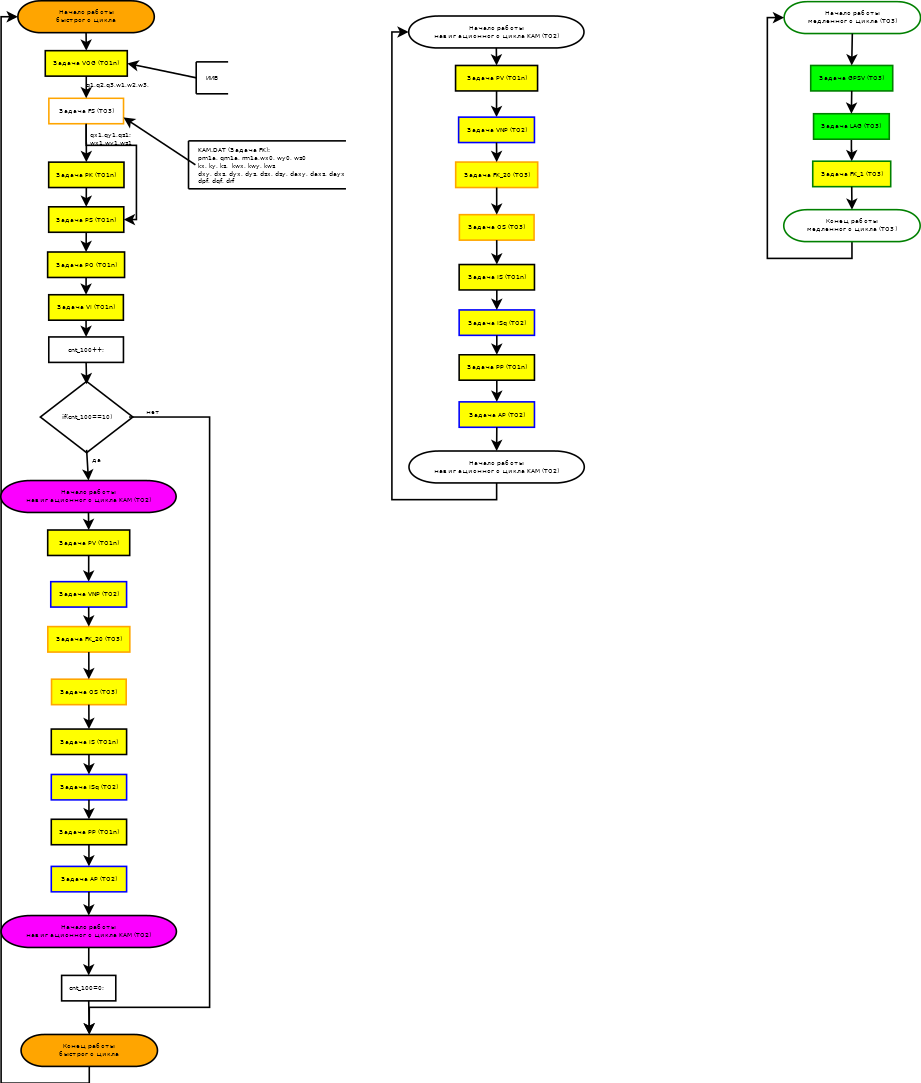
\includegraphics[width=1.0\linewidth]{images/general_scheme.png}
    \caption{Задачи программы}
    \label{fig:general_scheme}
\end{figure}
\subsection{Задача формирования сигналов FS}
Реализует следующие функции согласно схеме на Рис.~\ref{fig:FS}
\begin{figure}[H]
    \centering
    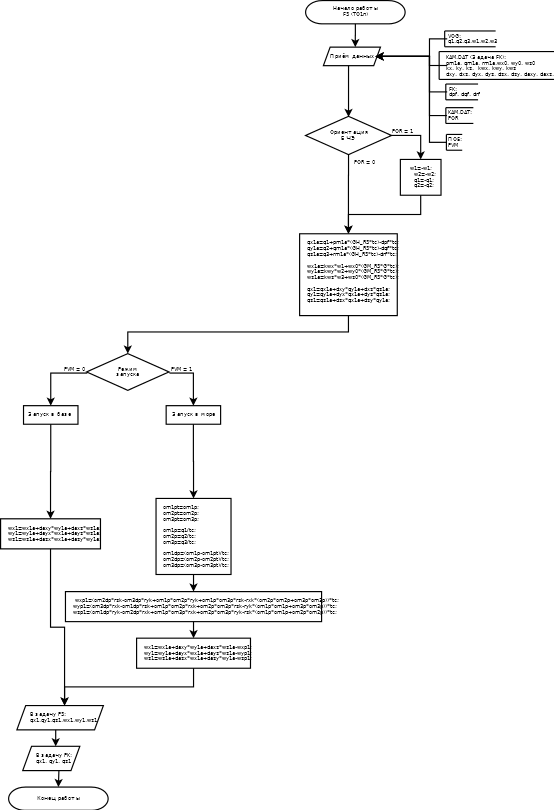
\includegraphics[width=0.8\linewidth]{images/FS.png}
    \caption{Задача FS}
    \label{fig:FS}
\end{figure}
\begin{itemize}
\item Принимает от задачи VOG сигналы - q1,q2,q3,w1,w2,w3 и формирует с учетом принятой модели  инструментальных погрешностей передаваемые в задачи PK и PS  
приращения угла поворота qx1,qy1,qz1 и кажущейся скорости wx1,wy1,wz1 в проекциях на оси БЧЭ.
\item Преобразует сигналы горизонтных каналов ВОГ- q1,q2  к осям обьекта при значении признака ориентации POR=1 в случае установки корпуса БЧЭ 
с поворотом на 180 относительно продольной оси объекта.
\item Осуществляет масштабирование, компенсацию аддитивных и мультипликативных составляющих модели  инструментальных погрешностей   
сигналов ВОГ и акселерометров с использованием задаваемых в случае необходимости в файле данных KAM.DAT корректур, а также меняющихся в запуске 
и  оцениваемых оптимальным фильтром Калмана ( ОФК ) составляющих дрейфов в осях БЧЭ:  
    \begin{itemize}
\item систематических ошибок  pm1a, qm1a, rm1a,wx0, wy0, wz0
\item масштабных коэффициентов kx, ky, kz,  kwx, kwy, kwz
\item невыставок  dxy, dxz, dyx, dyz, dzx, dzy, dаxy, dаxz, dаyx
\item оценки дрейфов dpf, dqf, drf
    \end{itemize}
\end{itemize}
\subsubsection{Входные и выходные данные задачи FS}
Входная информация
\begin{itemize}
    \item q1, q2, q3, w1,w2,w3- из задачи  VOG-приема сигналов БЧЭ
    \item pm1a,qm1a, rm1a, wx0, wy0, wz0, kwx, kwy, kwz, dxy, dxz, dyx, dyz, dzx, dzy, daxy, daxz, dayx, dayz, dazx, dazy - из файла данных kam.dat
    \item dpf, dqf, drf- из задачи  FK
\end{itemize}
Выходная информация
\begin{itemize}
    \item qx1, qy1, qz1- в задачу PK
    \item qx1,qy1,qz1,wx1,wy1,wz1-- в задачу PS
\end{itemize}
\subsection{Задача формирования скоростей опорного трехгранника OS}
Реализует следующие функции согласно упрощенной схеме на Рис.~\ref{fig:OS}
\begin{figure}[H]
    \centering
    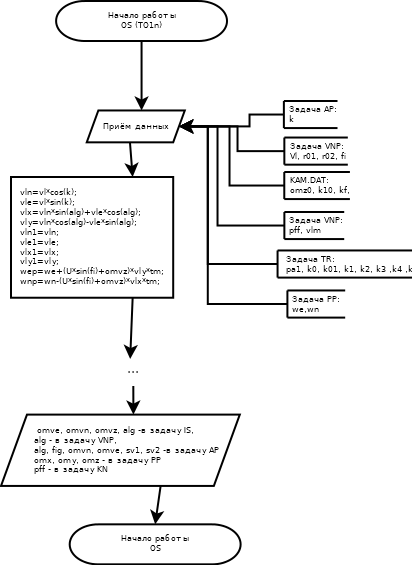
\includegraphics[width=0.8\linewidth]{images/OS_simple.png}
    \caption{Задача OS}
    \label{fig:OS}
\end{figure}
\begin{itemize}
    \item Формирует угловую скорость коррекции $\omega$  ( omx ,  omy,  omz ) -составляющие   угловой скорости   опорного   аналитического   
    трехгранника в проекциях  на собственные оси  - 
    по информации из задачи  PV о проекциях на горизонтальную плоскость аналитического трехгранника  приращения  кажущейся скорости БИНС 
    в осях аналитического  опорного трехгранника  за время  навигационного  цикла  ТМ.-- Wг (We, Wn, Wv).  
    \item Вычисляет по сигналу лага  VL  горизонтальные  составляющие скорости   обьекта в  проекциях  на оси  географического трехгранника VLE, 
    VLN с использованием курса К и -на оси  опорного   аналитического   трехгранника  VLX,  VLY с использованием курсового  угла  ALG 
    \item Компенсирует в  горизонтальных проекциях сигналов акселерометров кориолиссовы составляющие,  порождаемые вертикальной составляющей угловой 
    скорости  опорного   аналитического   трехгранника $omvz=U*sin(\phi)$  и  горизонтальными  составляющими скорости   обьекта в проекциях  на 
    оси  опорного   аналитического   трехгранника  для получения после их интегрирования  только составляющих скорости относительно Земли и  
    сравнения их с составляющими  сигнала  лага  в проекциях  на оси  опорного   аналитического   трехгранника   на предыдущем  шаге  
    VLX1,  VLY1  с  целью  формирования сигналов демпфирования   sv1,   sv2.
    \item В рабочем режиме (pa1=3) формирование сигналов демпфирования  sv1, sv2 и  абсолютных угловых скоростей опорного  аналитического  трехгранника  
    omve,  omvn,   omvz  производится  c  использованием корректур  dvx,   dvy,  выработанных  ОФК .
    \item Формирование  составляющих угловой скорости опорного   аналитического  трехгранника в проекциях  на собственные оси - выходные сигналы 
    задачи   OS-производится  с использованием корректур  db,   dg,   dalf,   выработанных  ОФК, что также обеспечивает демпфирование переходных 
    процессов, вызванных реальными начальными угловыми рассогласованиями , начальными отклонениями угловых скоростей, 
    ускорениями качки и инструментальными погрешностями.
    \item В конце задачи реализуется   контроль  уровня  угловых скоростей опорного трехгранника  и в случае  превышения  горизонтальными составляющими 
    угловых скоростей omx  или  omy  значения 2.e-4  рад.сек  (60  ͦ час)  включается счетчик циклов  cnf.
\end{itemize}
\subsubsection{Входные и выходные данные задачи OS}
Входная информация:
\begin{itemize}
    \item Vl, r01, r02, fi - из задачи  VNP
    \item pa1, k0, k01, k1, k2, k3 ,k4 ,k5 - из задачи   TR
    \item we,wn- из задачи   PP
    \item omz0, k10, kf, -из файла данных kam.dat
    \item k -из задачи AP
\end{itemize}
Выходная информация:
\begin{itemize}
\item omve, omvn, omvz, alg -в задачу IS, 
\item alg - в задачу VNP,
\item alg, fig, omvn, omve, sv1, sv2 -в задачу AP
\item omx, omy, omz - в задачу PP
\item pff - в задачу KN
\end{itemize}
\subsection{Задача вычисления параметров кватерниона РК}
Вычисляет, согласно упрощенной схеме на Рис.~\ref{fig:OS},  по  информации о приращениях за время быстрого цикла ТC  абсолютного угла поворота $\delta$ в проекциях на оси БЧЭ -  qx1, qy1, qz1, - из задачи  FS 
компоненты кватерниона mm (m0m, m1m, m2m, m3m), определяющего  ориентацию связанных осей БИНС относительно инерциального трехгранника путем численного 
интегрирования кинематического уравнения Пуассона.
\begin{figure}[H]
    \centering
    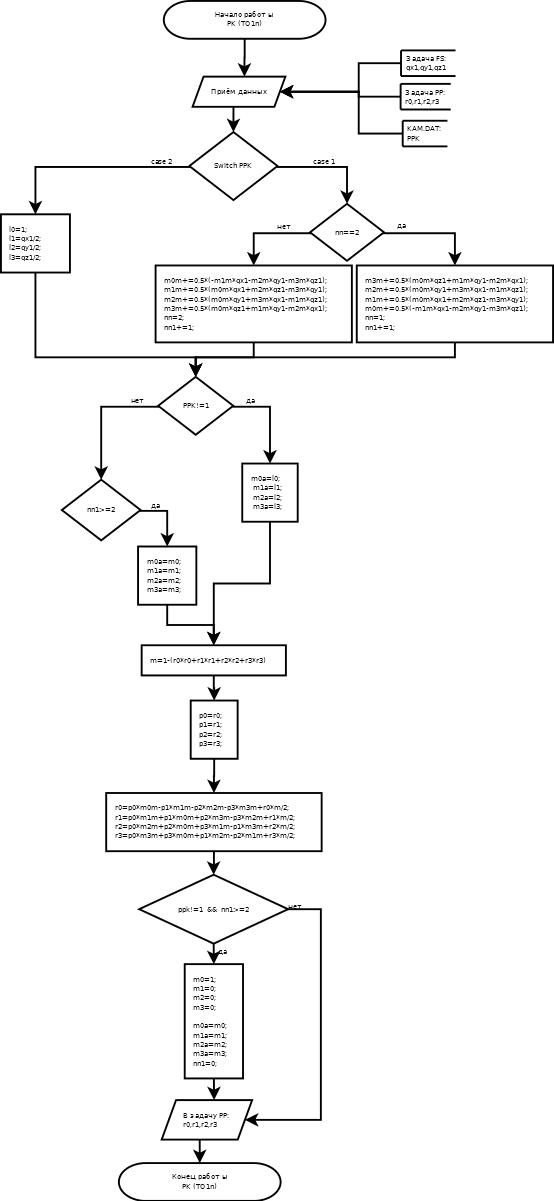
\includegraphics[width=0.7\linewidth]{images/PK.png}
    \caption{Задача PK}
    \label{fig:PK}
\end{figure}


\section{Схема алгоритма работы СПО «Кама-Надир»}
Файл приложения.
\end{uspd}
\end{document}
